
\subsection*{1.}

\(f(-3) = f(3) = 7\) sont les maximums de la fonction \(f\) sur \([-4\,;\,3]\).

\(f(1) = -25 \) est le minimum de la fonction \(f\) sur \([-4\,;\,3]\).

\subsection*{2.}

\(f\) fonction polynôme est dérivable sur \(\mathbb{R}\) et en particulier sur \([-4\,;\,3]\) :
\[
f'(x) = 3x^2 + 6x - 9 = 3(x^2 + 2x - 3).
\]

\subsection*{3.}

Le signe de \( f'(x) \) est celui de \( x^2 + 2x - 3 \). Pour ce trinôme :
\[
\Delta = 4 - 4 \times 1 \times (-3) = 16 = 4^2 > 0,
\]
ce trinôme a deux racines :
\[
x_1 = \frac{-2 + 4}{2} = 1, \quad \text{et} \quad x_2 = \frac{-2 - 4}{2} = -3.
\]
Remarque : La racine 1 était évidente.

\subsection*{4.}

On sait que ce trinôme est positif sauf sur l'intervalle \( ]-3\,;\,1[ \).

Il en résulte que sur l'intervalle \([-4\,;\,3]\) :
\begin{center}
\begin{tikzpicture}
\tkzTabInit[lgt=2.5, espcl=2]{$x$ / 1, {Signe de $f'(x)$} / 1, {$f$} / 2}{${-4}$, ${-3}$, ${1}$, ${3}$}
\tkzTabLine{,+,0,-,0,+,}
\tkzTabVar{-/{$0$},+/{$7$},-/{$-25$},+/{$7$}}{/}
\end{tikzpicture}
\end{center}
On retrouve bien les résultats de la question \textbf{1.}

\subsection*{5.}

On sait qu'une équation de la droite \( \mathcal{T} \), tangente à la courbe \( \mathcal{C} \) au point d'abscisse 0, est :
\[
y - f(0) = f'(0)(x - 0).
\]
Avec \( f(0) = -20 \) et \( f'(0) = -9 \), l'équation devient :
\begin{align*}
&y - (-20) = -9x \\
\iff &y = -9x - 20 \\
\iff &M(x\,;\,y) \in \mathcal{T}.
\end{align*}

